%--------------------------------------------------------------------------------------
% Este arquivo contém a sua funtamentação teórica
%--------------------------------------------------------------------------------------
\chapter{Fundamentação teórica}

\section{\textit{Background}}

Para um entendimento apropriado do estudo investigativo, são discutidos aqui conceitos básicos do processamento digital de imagens, como espaços de cores, pré-processamento e técnicas de inferência para determinação de um atributo desejado. 

\subsection{Espaços de cores}

Um espaço de cores é um modelo matemático utilizado para a representação de uma cor através de três ou mais componentes (SHAIK et al., 2015). Um espaço de cor pode ser orientado a um hardware específico, como o modelo RGB (\textit{Red, Green, Blue}), para exibição em monitores coloridos ou aquisição por uma câmera digital. Entretanto, este espaço de cor não permite uma interpretação humana exata de como a cor é composta. Por outro lado, espaços de cores como o L*a*b* e HSV (\textit{Hue}, \textit{Saturation}, \textit{Value}) permitem uma descrição mais natural. 

\subsubsection{RGB}

Este modelo é baseado nas três cores primárias, a partir das quais ele é nomeado: vermelho (\textit{Red}), verde (\textit{Green}) e azul (\textit{Blue}). Ele é representado por um sistema de coordenadas 3D, em que cada cor é dada por um vetor que se origina na origem. Os três elementos do vetor consistem nas intensidades de cada cor primária, e assim, uma imagem RGB é representada por três matrizes, cada uma contendo as intensidades do respectivo canal (R, G, B) para todos os pixels da imagem. Quando as três cores são combinadas em suas intensidades máximas, o olho humano percebe a cor resultante como branca. Por outro lado, quando as três intensidades são nulas, tem-se a cor preta como resultante. No subespaço RGB, mostrado na Figura \ref{img:rgb_cube}, o segmento de reta que une as cores branca e preta consiste na escala de cinza, onde as intensidades dos três canais são iguais. Os demais vértices do cubo correspondem às cores primárias e secundárias (SONKA; HLAVAC; BOYLE, 2014).  

\begin{figure}[H]
\centering
    \caption{\label{img:rgb_cube} Subespaço de cores RGB.}
    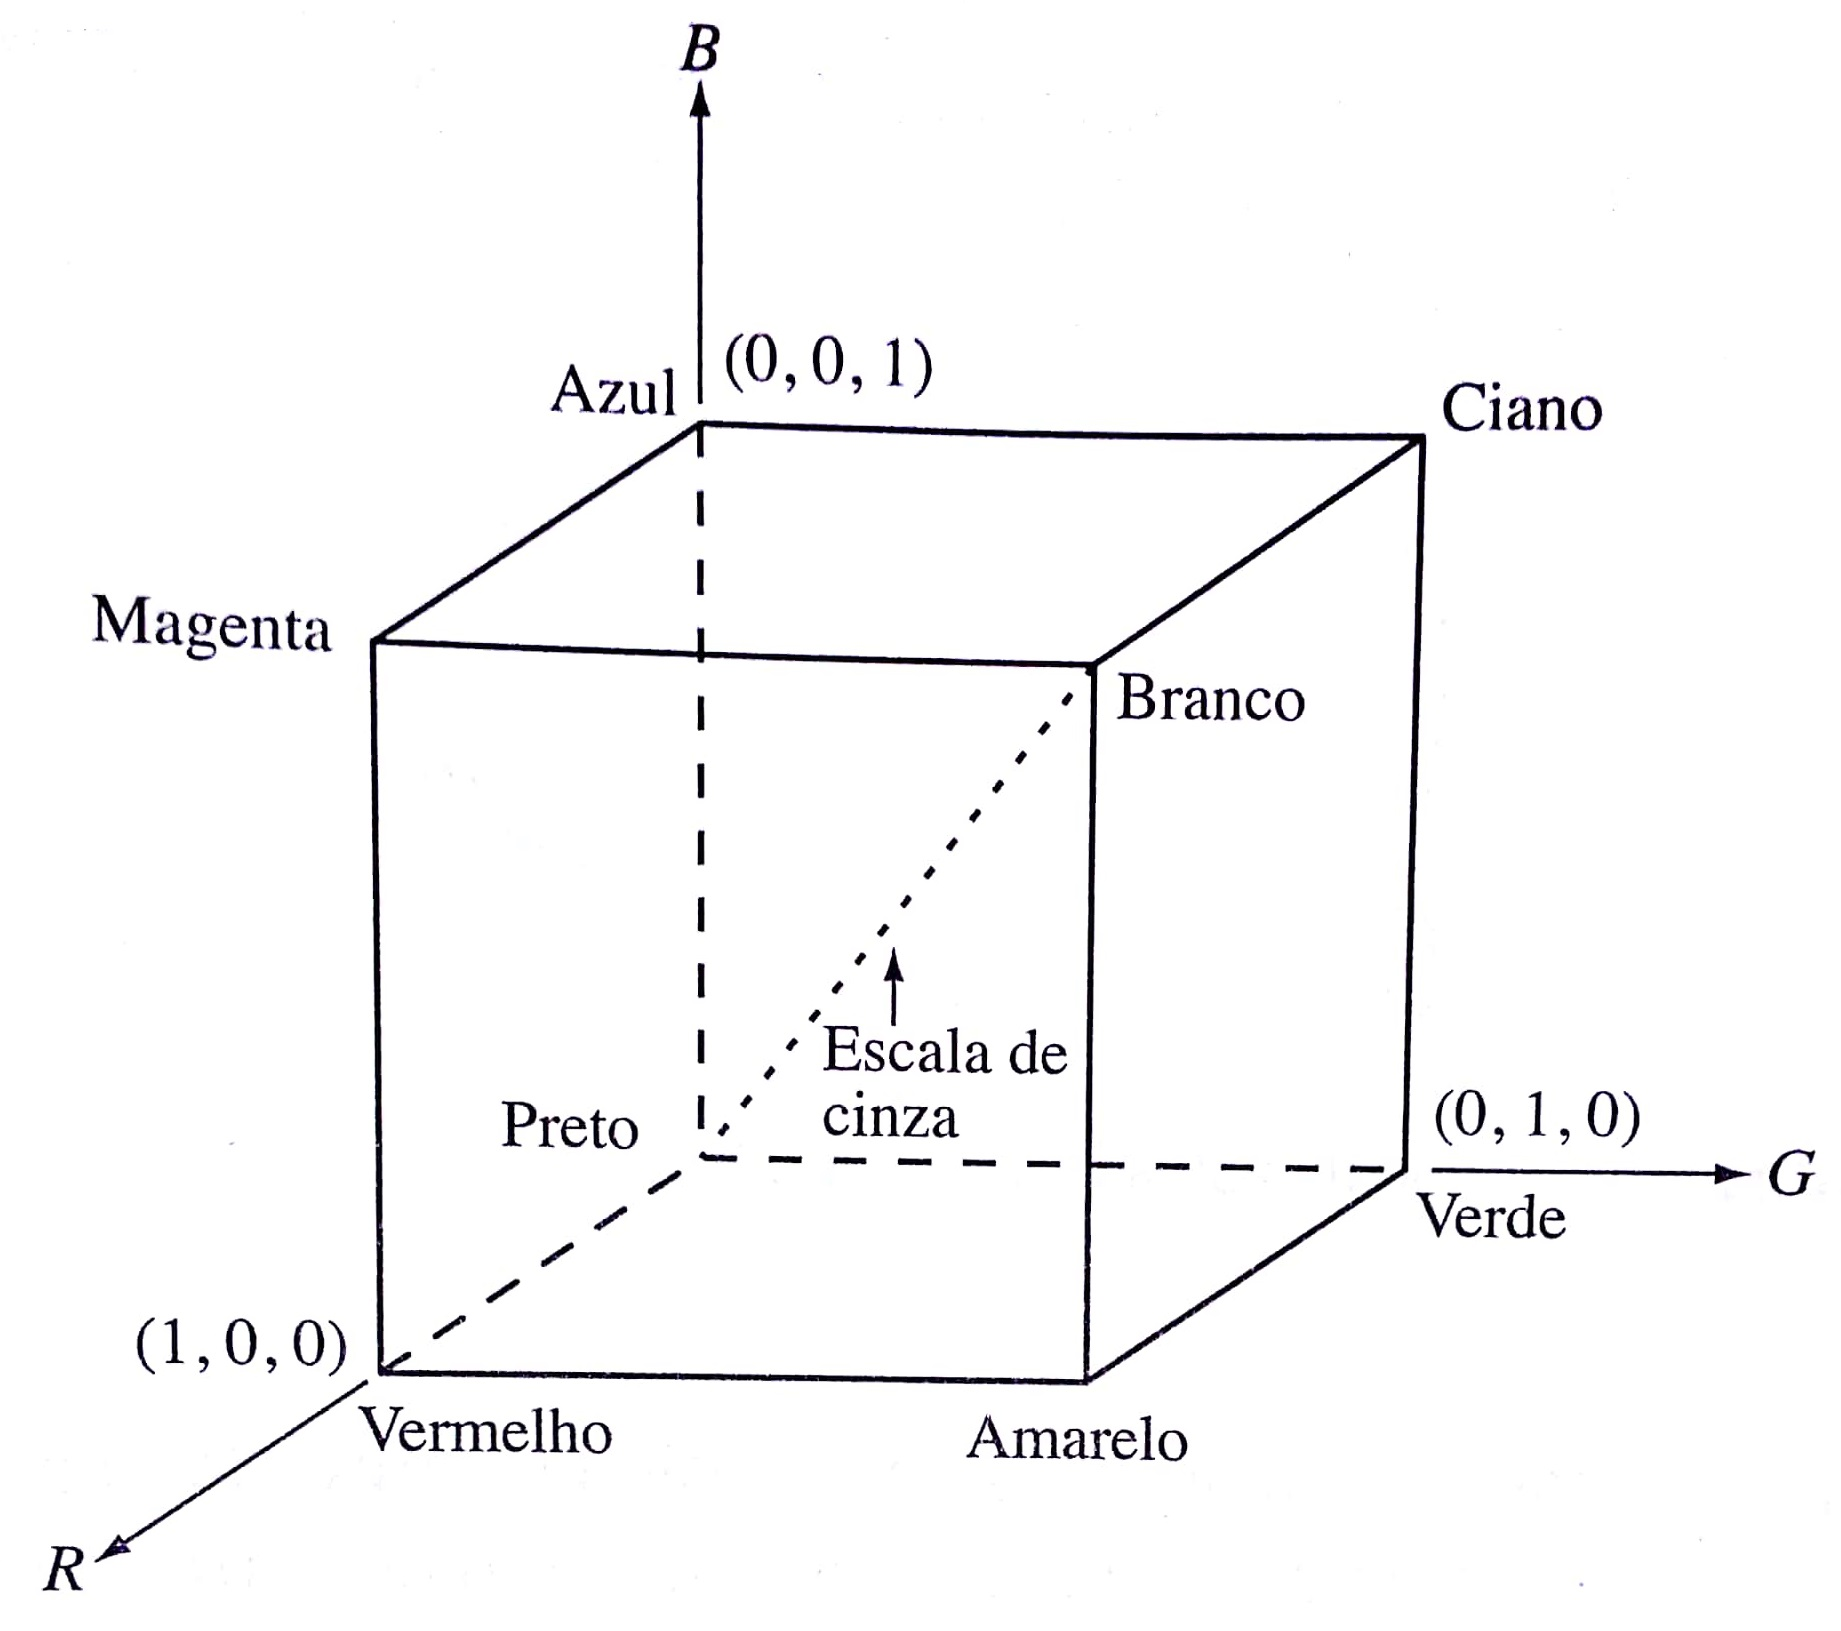
\includegraphics[scale=0.09]{img/rgb_cube}
    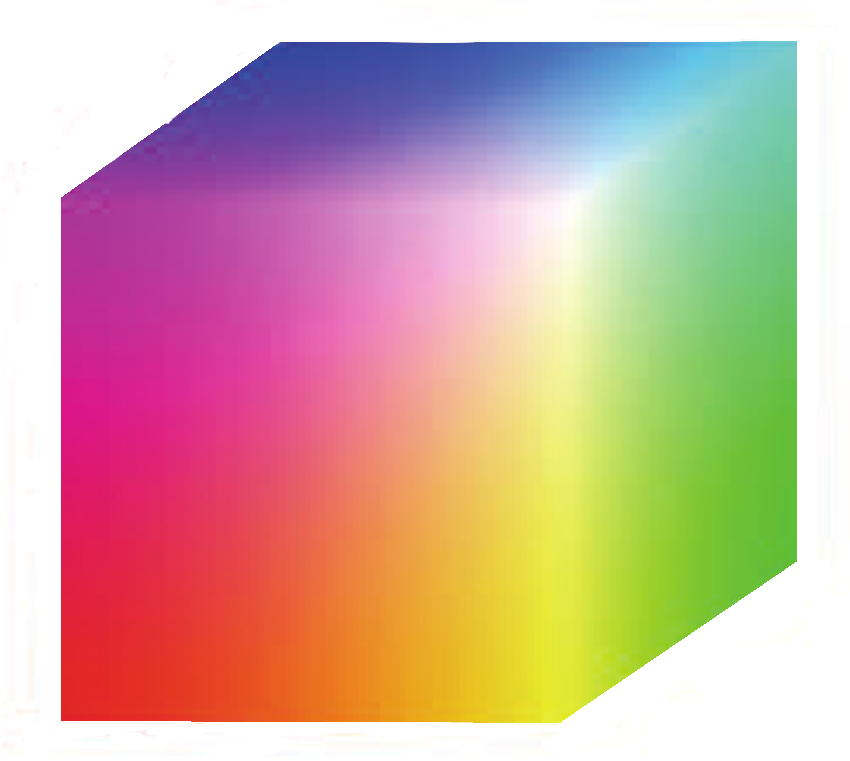
\includegraphics[scale=0.15]{img/rgb_cube2}
    \legend{\textbf{Fonte: } (GONZALEZ; WOODS, 2009; DATAR; JONES; SMITH JR., 2005).}
\end{figure}

\subsubsection{L*a*b*}

Este espaço de cores, também chamado de CIE-Lab, emprega como componentes a luminosidade (L*), que varia entre 0 (preto)  e 100 (branco) e os canais “vermelho-verde” (a*) e “amarelo-azul” (b*). Estes últimos canais representam a variação da cor entre verde até vermelho e amarelo até azul respectivamente. A representação de uma imagem neste sistema de cores é obtida a partir da conversão do espaço RGB para o XYZ inicialmente, através da equação (\ref{eq:xyz}):

\begin{equation} \label{eq:xyz}
	\begin{bmatrix}
		X \\
		Y \\
		Z \\
	\end{bmatrix} =
	\begin{bmatrix}
		0,4125 & 0,3576 & 0,1804 \\
		0,2127 & 0,7152 & 0,0722 \\
		0,0193 & 0,1192 & 0,9502
	\end{bmatrix}
	\begin{bmatrix}
		R \\
		G \\
		B \\
	\end{bmatrix}
\end{equation}

Após essa conversão, os valores L*, a* e b* são obtidos a partir das equações (\ref{eq:lab1}), (\ref{eq:lab2}) e (\ref{eq:lab3}) (KAUR; KRANTHI, 2012), em que ($X_b$,  $Y_b$,  $Z_b$) é a coordenada que representa a cor branca neste espaço de cor.  

\begin{equation} \label{eq:lab1}
	L* =
		\begin{cases}
			116*(\frac{Y}{Y_b})^{\frac{1}{3}} - 16 & onde \ \frac{Y}{Y_b} > 0,008856 \\
			903,3 									& onde \ \frac{Y}{Y_b} \leq 0,008856
		\end{cases}
\end{equation}

\begin{equation} \label{eq:lab2}
	a* = 500 * 
		\begin{bmatrix}
			\frac{X^\frac{1}{3}}{X_b} - \frac{Y^\frac{1}{3}}{Y_b}
		\end{bmatrix}
\end{equation}

\begin{equation} \label{eq:lab3}
	b* = 200 *
		\begin{bmatrix}
			\frac{X^\frac{1}{3}}{X_b} - \frac{Z^\frac{1}{3}}{Z_b}
		\end{bmatrix}
\end{equation}

\subsubsection{HSV}

O sistema HSV, também conhecido como HSB, possui como componentes a matiz (\textit{Hue}), saturação (\textit{Saturation}) e valor ou brilho (\textit{Value} ou \textit{Brightness}), sendo capaz de descrever uma cor de uma forma mais intuitiva para os humanos (NADAFZADEH; MEHDIZADEH; SOLTANIKAZEMI, 2018).

A matiz é associada à cor dominante em uma mistura de cores, da forma como é percebida por um humano. Ela é descrita em graus, variando entre 0º e 360º, de acordo com sua localização na roda de cores, conforme a Figura \ref{img:hsv_hex}. A saturação mede o grau de diluição de uma cor pura por luz branca, sendo estimada de acordo com a distância da cor até a origem do cone, que representa a cor branca. Por fim, o valor ou brilho indica a quantidade de luz na combinação, sendo obtida a partir da distância da cor a partir do preto até o branco. Tanto a saturação quanto o valor/brilho possuem valores variando entre 0 e 1 (DORJ; LEE; YUN, 2017).

\begin{figure}[H]
\centering
    \caption{\label{img:hsv_hex} Representação 3D do espaço de cores HSV.}
    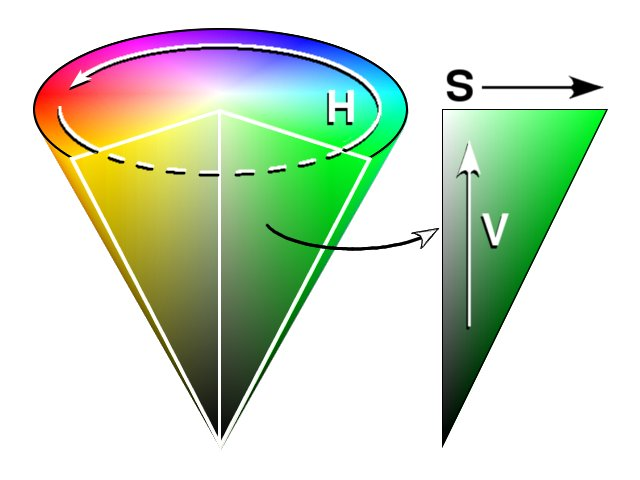
\includegraphics[scale=0.25]{img/hsv_hex}
    \legend{\textbf{Fonte: } (Wikipedia, 2019).}
\end{figure}

Pode ser realizada a conversão de uma imagem no espaço de cores RGB para HSV, de forma a se obter uma melhor descrição da mesma, através das seguintes equações: 

\begin{equation} \label{eq:hsv1}
	H = \begin{cases}
			\theta, 		& se \ B \leq G \\
			360 - \theta, 	& se \ B > G
		\end{cases}
\end{equation}

\begin{equation} \label{eq:hsv2}
	\theta = \arccos{
		\Bigg\{ \frac{\frac{1}{2}[(R - G) + (R - B)]}{\sqrt{[(R - G)^2 + (R - G)*(G - B)]}}
	}
\end{equation}

\begin{equation} \label{eq:hsv3}
	S = 1 - \frac{3}{R + G + B}[mín(R,G,B)]
\end{equation}

\begin{equation} \label{eq:hsv4}
	V = \frac{1}{3}(R + G + B)
\end{equation}

\subsection{Pré-processamento de imagens}

A seguir estão descritas algumas das técnicas de pré-processamento mais comuns. Elas subdividem-se quanto ao domínio em que atuam, podendo ser realizadas no domínio espacial, em que as técnicas são aplicadas nos pixels diretamente, ou no domínio da frequência, em que os métodos são realizados no espectro de frequência da imagem (BEDI; KHANDELWAL, 2013). 

\subsubsection{Filtro da mediana}

A filtragem da mediana consiste em uma operação não linear realizada no domínio espacial. Através dela o ruído de uma imagem é removido enquanto as bordas são preservadas, pois ele não é tão sensível a valores extremos. Para realizar a filtragem, move-se uma janela de tamanho predefinido pixel a pixel, de forma que cada valor seja substituído pela mediana dos valores dos pixels contidos na janela (HEMALATHA; SUMATHI, 2016). Este filtro é comumente empregado para imagens com ruído do tipo \textit{salt and pepper}, que consiste em pixels aleatórios de cor branca ou preta, conforme mostra a Figura \ref{img:median_filter}.

\imagem{0.5}{median_filter}{Remoção de ruído \textit{salt and pepper} por um filtro da mediana com tamanho da janela igual a 3x3.}{(MathWorks Inc., 2006).}

\subsubsection{Operações de abertura e fechamento (\textit{Opening and closing operations})}

As operações de abertura e fechamento são do tipo morfológicas, em que são realizadas transformações em uma imagem, normalmente binária, com base no formato do objeto nela contido. Elas se diferem quanto à ordem em que as operações de erosão e dilatação, também morfológicas, são realizadas em uma imagem.

Nestas duas operações, um \textit{kernel}, que consiste em uma janela de tamanho predefinido preenchida com 0s ou 1s, percorre a imagem original, substituindo o valor de um pixel caso os pixels contidos na janela sejam todos iguais a 1, no caso da erosão, ou pelo menos um deles seja igual a 1, no caso da dilatação. Na Figura \ref{img:eros_dilat} são mostrados os efeitos do uso da erosão e dilatação em uma mesma imagem.

\begin{figure}[H]
\centering
    \caption{\label{img:eros_dilat} Utilização da erosão e dilatação em uma imagem (a) Imagem original (b) Imagem erodida (c) Imagem dilatada.}
    \subcaptionbox{}{
\includegraphics[scale=0.6]{img/j.png}}
    \subcaptionbox{}{
\includegraphics[scale=0.6]{img/j_eros.png}}
    \subcaptionbox{}{
\includegraphics[scale=0.6]{img/j_dilat.png}}
    \legend{\textbf{Fonte: } (OpenCV, 2019).}
\end{figure}

A operação de abertura realiza a erosão seguida de dilatação, resultando na eliminação de ruídos pontuais enquanto mantém as formas do objeto. Por outro lado, a operação de fechamento primeiro aplica a dilatação e depois a erosão, o que, além de também manter o contorno do objeto, contribui para o preenchimento de pequenos buracos (ARCO et al; 2015). A Figura \ref{img:morph_op} mostra o resultado da utilização destas operações. 

\begin{figure}[H]
\centering
    \caption{\label{img:morph_op} Operações morfológicas aplicadas na letra "j" (a) Abertura (b) Fechamento.}
    \subcaptionbox{}{
\includegraphics[scale=0.6]{img/opening.png}}
    \subcaptionbox{}{
\includegraphics[scale=0.6]{img/closing.png}}
    \legend{\textbf{Fonte: } (OpenCV, 2019).}
\end{figure}

\subsection{Segmentação de imagens}

O objetivo da segmentação consiste em dividir a imagem em subconjuntos disjuntos, de forma a obter apenas a região desejada. A segmentação torna-se simples quando na imagem em questão há objetos contrastantes em um fundo uniforme. Dessa forma, pode-se utilizar uma abordagem baseada no histograma da imagem, que fornece a frequência dos níveis de intensidade dela (GONZALEZ; WOODS, 2009).

\subsubsection{Limiarização}

A limiarização é o método de segmentação mais simples, rápido e pouco custoso existente. Ela é utilizada em imagens em que os objetos nela presentes possuem uma absorção de luz uniforme ao longo de suas superfícies, de forma que, a partir de um valor limiar, ou \textit{threshold}, é possível fazer a separação completa dos objetos da imagem (SONKA; HLAVAC; BOYLE, 2008).

Assim, dada uma imagem $f(i, j)$, obtém-se uma imagem segmentada $g(i, j)$ conforme a equação abaixo, considerando um \textit{threshold} T dado:

\begin{equation} \label{eq:thrd}
	g(i, j) =
		\begin{cases}
			1, & se \ f(i, j) \geq T, \\	
			0, & se \ f(i, j) < T
		\end{cases}
\end{equation}

Na Figura \ref{img:thresholding} é mostrado o resultado da limiarização simples aplicada numa imagem gradiente em escala de cinza. Como esta imagem é representada em 8 bits e seus valores de intensidade  variam entre 0 e 255 ($2^8$), ao utilizar um limiar igual a 127, a imagem resultante consiste em duas metades cujos pixels são iguais a 0 e 1. 

\begin{figure}[H]
\centering
    \caption{\label{img:thresholding} Limiarização simples aplicada em uma imagem, com \textit{threshold} igual a 127. À esquerda, a imagem gradiente, cuja intensidade varia entre 0 e 255. À direita, o resultado da limiarização.}
    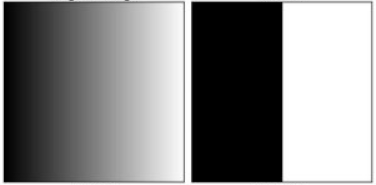
\includegraphics[scale=0.5]{img/thresholding.png}
    \legend{\textbf{Fonte: } (OpenCV, 2003).}
\end{figure}

\subsubsection{Segmentação de Otsu}

Esta técnica de segmentação é eficaz para imagens bimodais, cujos histogramas possuem dois picos. Este método calcula um limiar ótimo que se localiza aproximadamente no meio dos dois picos (GONZALEZ; WOODS, 2009). O algoritmo de Otsu busca um \textit{threshold} t tal que a variância entre uma mesma classe é minimizada. No contexto de uma imagem, uma classe seria o objeto de estudo ou o plano de fundo. A função a ser minimizada é dada por:

\begin{equation} \label{eq:otsu}
	\sigma_w^2(t) = q_1(t)\sigma_1^2(t) + q_2(t)\sigma_2^2(t)
\end{equation}

Em que $q_1(t)$ e $q_2(t)$ são as probabilidades das classes associadas ao limiar t, dadas por:

\begin{equation}
	q_1(t) = \sum_{i=1}^t{P(i)} \;\;\;\;\;\; q_2(t) = \sum_{i=t+1}^I{P(i)}
\end{equation}

Em que $P(i)$ é o histograma da imagem, tratado como função de densidade de probabilidade, e I é o nível máximo de intensidade da imagem. $\sigma_1^2(t)$ e $\sigma_2^2(t)$ são as variâncias das classes, dadas por:

\begin{equation}
	\sigma_1^2(t) = \sum_{i=1}^t{[i-\mu_1(t)]^2\frac{P(i)}{q_i(t)}} \;\;\;\; \sigma_2^2(t) = \sum_{i=t+1}^I{[i-\mu_1(t)]^2\frac{P(i)}{q_2(t)}}
\end{equation}

Em que:

\begin{equation}
	\mu_1(t) = \sum_{i=1}^t{i\frac{P(i)}{q_i(t)}} \;\;\;\; \mu_2(t) = \sum_{i=t+1}^I{i\frac{P(i)}{q_2(t)}}
\end{equation}

Na Figura \ref{img:otsu} é mostrada uma imagem original e o resultado da segmentação de Otsu.

\begin{figure}[H]
\centering
    \caption{\label{img:otsu} Segmentação de Otsu. À esquerda, a imagem original. À direita, a imagem segmentada pelo algoritmo.}
    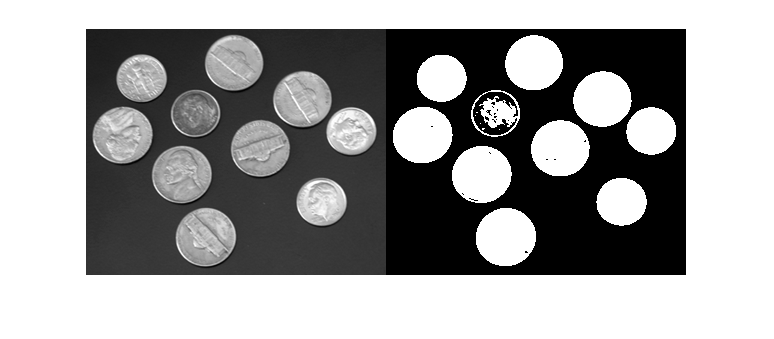
\includegraphics[scale=0.5]{img/otsu.png}
    \legend{\textbf{Fonte: } (Mathworks Inc., 2006).}
\end{figure}

% \imagem{0.5}{otsu}{Segmentação de Otsu. À esquerda, a imagem original. À direita, a imagem segmentada pelo algoritmo de Otsu.}{(MathWorks Inc., 2006).}

\subsection{Técnicas de inferência}

As técnicas aqui apresentadas são empregadas para a predição de uma variável de saída desejada com base nas variáveis de entrada fornecidas, através de modelos supervisionados de regressão ou classificação, em que a variável de saída é quantitativa ou qualitativa, respectivamente (DA SILVA; PERES; BOSCARIOLI, 2017). Para tal, deve-se utilizar um conjunto de amostras de treinamento, em que as variáveis de entrada e saída são conhecidas, para a construção de um modelo matemático que extraia padrões a partir dos dados fornecidos. Assim, tendo modelado o relacionamento entre as variáveis, pode-se realizar a predição para novas amostras, em que sua variável de saída é desconhecida (GAMA, 2015).

\subsubsection{Regressão linear múltipla}

A MLR (\textit{Multiple Linear Regression}) é um método de regressão que assume um relacionamento linear entre os atributos de entrada e o de saída (JAMES et al., 2013). Ela é uma extensão da regressão simples, que emprega apenas uma variável de entrada, e apresenta um bom desempenho quando empregada em um conjunto de dados que não possua ruído ou colinearidade entre os atributos. A equação que descreve a MLR é dada por:

\begin{equation} \label{eq:mlr}
	Y = \beta_0 + \beta_1 X + \epsilon
\end{equation}

Em que $Y$ é o vetor de atributo alvo, $\beta_0$ é o intercepto, $\beta_1$ é o vetor de inclinações da equação, $X$ é o vetor de atributos e $\epsilon$ é o erro aleatório. 

Os parâmetros da MLR são normalmente estimados pelo método dos mínimos quadrados, que busca minimizar a soma do quadrado dos resíduos (RSS – \textit{Residual Sum of Squares}), dada pela equação abaixo:

\begin{equation} \label{eq:rss}
	RSS = e_1^2 + e_2^2 + ... + e_n^2
\end{equation}

Em que $e_1^2$, $e_2^2$, ..., $e_n^2$ correspondem à diferença entre o valor previsto pelo modelo e o valor real para as $n$ amostras. 

\subsubsection{\textit{Random Forest}}

A \textit{Random Forest} consiste em uma técnica \textit{ensemble} não linear, em que uma variável qualitativa ou quantitativa é determinada através de uma combinação de modelos de árvores de decisão (FRIEDMAN; HASTIE; TIBSHIRANI, 2001). A relação entre as variáveis de entrada e a de saída é modelada através de um conjunto de regras de decisão, construídas por divisões binárias e recursivas dos dados de treinamento. Cada regra de decisão utiliza uma única variável de entrada para a divisão dos dados, sendo ela selecionada a partir de um subconjunto aleatório de todas as variáveis. Um modelo de regressão é então construído a partir das variáveis selecionadas e o erro RSS é calculado (HUTENGS; VOHLAND, 2016). As regras de decisão e consequentemente as variáveis de entrada, são selecionadas visando a minimização desse erro. Assim, a \textit{Random Forest} permite a determinação das variáveis mais significativas para a predição da variável de saída. 

O valor previsto resultante será a média dos resultados obtidos para cada árvore de decisão. Para evitar a correlação entre as árvores, elas são construídas a partir de subconjuntos não disjuntos dos dados de entrada, o que torna o modelo resultante mais estável, robusto e preciso (BREIMAN, 2001).

\subsection{Avaliação do desempenho de modelos}

Para a avaliação da capacidade preditiva dos modelos, é comumente utilizada a estratégia de validação cruzada k-\textit{fold} (k-\textit{fold cross validation}). Ela é empregada para assegurar que não há um sobreajuste (\textit{overfitting}) no modelo, através da divisão do conjunto de dados em k subconjuntos disjuntos, com uma alocação das amostras para o conjunto de treinamento ou teste (DA SILVA; PERES; BOSCARIOLI, 2017). Assim, um dos subconjuntos é utilizado como teste e os k-1 demais para o treinamento, de forma que o modelo realize a predição para dados desconhecidos. Este procedimento é repetido k vezes, alterando os subconjuntos a cada vez.

As predições resultantes podem então ser avaliadas através de métricas, tais como o coeficiente de correlação e RMSE, empregadas nos artigos em que a regressão foi realizada. Estes indicadores medem, respectivamente, o grau de dependência entre as variáveis de entrada e saída e a magnitude média dos erros estimados (ALVES; VECCHIA, 2011), conforme as equações abaixo:

\begin{equation} \label{eq:r}
	R = \frac{\sum_{i=1}^n (x_i - \overline{x})(y_i - \overline{y})}{\sqrt{\sum_{i=1}^n(x_i - \overline{x})^2} \sqrt{\sum_{i=1}^n (y_i - \overline{y})^2}}
\end{equation}

\begin{equation} \label{eq:rmse}
	RMSE = \sqrt{\frac{1}{n} \sum_{i=1}^n (y_i - \hat{y}_i)^2}
\end{equation}

Em que $x_i$ é o valor da variável de entrada, $\overline{x}$ é a média dos valores de $x$, $y_i$ é o valor real da variável de saída, $\overline{y}$ é a média dos valores de $y$, $n$ é o número de amostras e $\hat{y}_i$ é o valor previsto para a variável de saída.

\section{Trabalhos relacionados}

A seguir são discutidos dez artigos \textit{(Apêndice A)} em que é empregado o processamento digital de imagens para determinação de atributos de qualidade em mangas. O estudo investigativo foi conduzido de acordo com as técnicas e métricas empregadas pelos autores, assim como os atributos extraídos das imagens das mangas. 

Teoh e Syaifudin (2007) propuseram em seu trabalho a determinação do peso de mangas da variedade Chokanan\footnote{\label{ftnote:chokanan}Variedade originária da Tailândia, caracterizada por frutos compridos com pontas cônicas, polpa sem fibra, pele grossa e alta resistência a doenças.} através de imagens obtidas por uma câmera digital. 100 amostras aleatórias de mangas maduras e verdes foram coletadas e divididas entre treinamento e teste (50 para cada conjunto). Os valores reais do peso das mangas foram obtidos por uma balança digital. As mangas foram inicialmente imersas em água e limpas usando uma esponja e, após isso, foram postas em uma superfície preta e tiveram suas imagens tiradas por uma câmera de 0.3m mm/pixel de resolução, que foi situada a 22 cm acima do fruto, com uma fonte de luz de cada lado do aparelho. 

Para o pré-processamento das imagens, inicialmente empregou-se o filtro da mediana de tamanho 15x15 para correção de inconsistências nas imagens devido à iluminação não uniforme. As imagens foram então segmentadas por limiarização, através da análise do histograma bimodal. A Figura \ref{img:img_art_1} mostra os resultados das etapas empregadas pelos autores. A partir da imagem binária foi contado o número de pixels da região da manga, de forma que através desta variável independente o peso da respectiva manga fosse determinado. Um modelo de regressão linear foi então construído utilizando para tal 50 amostras de manga, enquanto que as demais foram empregadas para o teste do modelo, por intervalos de confiança a 95\%. A abordagem proposta pelos autores mostrou-se precisa, alcançando um coeficiente de correlação igual a 97,69\% e erro médio igual a 3,76\%. 

\begin{figure}[!htb]
\centering
    \caption{\label{img:img_art_1} Etapas empregadas pelos autores.}
    \subcaptionbox{Imagem original}{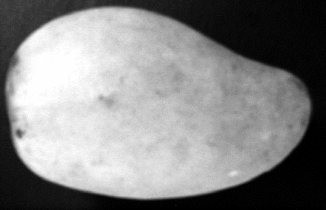
\includegraphics[scale=0.38]{img/art11}}
    \subcaptionbox{Imagem filtrada}{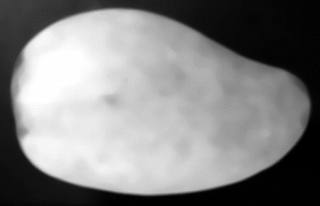
\includegraphics[scale=0.39]{img/art12}}
    \subcaptionbox{Imagem segmentada}{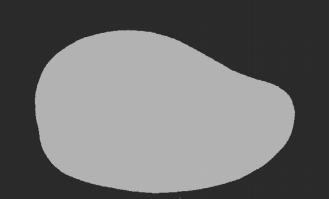
\includegraphics[scale=0.4]{img/art13}}
    \legend{\textbf{Fonte: } (TEOH; SYAIFUDIN, 2007).}
\end{figure}

No estudo de Nandi, Tudu e Koley (2014), mangas de diferentes variedades foram separadas quanto aos dias restantes até o apodrecimento das mesmas. Foram obtidas 1350 amostras de cinco diferentes variedades e provenientes de três pomares, coletadas em três lotes com um intervalo de uma semana entre eles, sendo que em cada lote havia 90 mangas de cada variedade. As mangas foram utilizadas como entrada no sistema automatizado até o dia do apodrecimento delas, resultando em 16400 imagens. Em cada dia, três especialistas determinaram os dias restantes até a data de expiração. As imagens tiradas foram divididas em quatro grupos quanto aos dias restantes até que a respectiva manga apodrecesse (12 dias restantes, 9 até 12 dias, 5 até 8 dias e 1 até 4 dias).

Para a classificação automática das mangas, foi desenvolvido um sistema composto por uma correia transportadora, motor, válvulas solenoides, controladora lógica, câmara de aquisição de imagens e um computador. Uma câmera com Dispositivo de Carga Acoplada (CCD, \textit{Charge-coupled Device}) com resolução 640x480 e frame rate igual a 30 \textit{frames}/s foi posicionada no interior da câmara, iluminada artificialmente, sendo que as imagens foram enviadas ao computador pela porta USB. As mangas eram dispostas na correia transportadora, de forma que, através de válvulas solenoides, elas fossem posicionadas no recipiente relativo à classe prevista. 

Inicialmente os frames adequados foram pré-processados por um filtro \textit{deblurring} de Wiener e filtro da mediana. Após isso, foram convertidos para uma imagem binária e as bordas foram traçadas por um algoritmo baseado em código em cadeia. As imagens das mangas foram então alinhadas em posição vertical para a posterior extração dos atributos. Os autores utilizaram apenas o espaço RGB para tal, levando em consideração o processo de maturação da manga e seu efeito nas regiões da fruta. Assim, as variáveis escolhidas foram as médias dos valores R, G e B da manga inteira e das três regiões (cume, equatorial e haste ou \textit{apex}, \textit{equator} e \textit{stalk}), o gradiente dos três canais ao longo do eixo longitudinal, diferença das médias R, G e B da manga inteira e das três regiões. A Figura \ref{img:art2} exibe as regiões da manga consideradas para a extração de atributos.

\imagem{0.5}{art2}{Imagem pré-processada e segmentada de uma manga, com suas regiões marcadas.}{(NANDI; TUDU; KOLEY, 2014).}

O melhor subconjunto de variáveis foi obtido por eliminação recursiva de atributo (RFE) aliada à SVM, onde se obteve um \textit{ranking} para cada variável. A SVM foi computada iterativamente, incrementando uma variável por vez, obtida a partir de uma lista decrescente de \textit{ranking}. A classificação foi realizada por um ensemble de 7 SVMs binárias, em que cada uma realizava a separação de uma combinação diferente de 2 classes. Os parâmetros ótimos das SVMs e o melhor \textit{kernel} foram obtidos por validação cruzada 6-\textit{fold} através de uma busca em \textit{grid}. Após a classificação ser feita, o computador comunica-se com o controlador lógico que ativa a válvula correspondente à classe prevista e controla a velocidade da correia transportadora. 

O sistema proposto pelos autores apresentou resultados satisfatórios, alcançando uma acurácia média igual a 96\% ao empregar a SVM Gaussian RBF, sendo que o subconjunto de variáveis obtido pelo método RFE continha predominantemente atributos derivados do canal R.

Zheng e Lu (2012) propuseram um método para classificação de mangas quanto a seu estágio de escurecimento empregando a LS-SVM. As 90 mangas coletadas de um supermercado possuíam diferentes graus de escurecimento. Elas foram classificadas visualmente por um perito em três diferentes classes: fresca sem escurecimento, escurecimento moderado e escurecimento severo. Foram então tiradas três imagens de cada manga através de uma câmera digital Canon EOS 50 D, sob iluminação solar. Antes da extração dos atributos, cada imagem foi pré-processada através da sua subtração pelo fundo.

Os atributos extraídos foram os valores médios dos canais L*, a*, b*, e as dimensões fractais dos frutos, que consistem em descritores geométricos das imagens. Estas foram calculadas por três diferentes técnicas: dimensão de contagem de caixa (BCD, \textit{Box Counting Dimension}), dimensão de correlação (CD, \textit{Correlation Dimension}) e dimensão de dilatação (DD, \textit{Dilation Dimension}). 

Na técnica BCD, o espaço euclidiano que contém a imagem é dividido em um \textit{grid} de caixas de tamanho r, que, ao ser diminuído progressivamente, resulta em diferentes quantidades de caixas não vazias, dada por $N(r)$. O valor da variável BCD é então dado por:

\begin{equation} \label{eq:bcd}
	BCD = \lim_{r->0}\frac{\log{N(r)}}{\log{(1/r)}}
\end{equation}

De forma semelhante, na variável DD cada pixel da borda da imagem é substituído por um círculo de diâmetro r que aumenta progressivamente, resultando em diferentes valores para o comprimento de borda $L(r)$ de cada círculo. Assim, o valor DD é encontrado através da Equação \ref{eq:dd}.

\begin{equation} \label{eq:dd}
	DD = \lim_{r->0}{\frac{\log{L(r)}}{\log{(1/r)}}}
\end{equation}

Por fim, CD é uma medida de dimensionalidade, calculada através da \ref{eq:cd}:

\begin{equation} \label{eq:cd}
	CD = \lim_{r->0}{\frac{\log{C(r)}}{\log{(1/r)}}}
\end{equation}

Em que $C(r)$ é dada por:

\begin{equation} \label{eq:c}
	C(r) = \lim_{n->\inf}\frac{1}{N^2} \sum_{j=1}^N \sum_{i=j+1}^N \theta (r - \|R_i - R_j\|)
\end{equation}

Em que $r$ é uma distância limiar, $N$ é o número de pontos, $\theta$ é a função de \textit{Heaviside} e $R$ representa os pontos.

Assim, três diferentes modelos LS-SVM foram computados: um que utiliza apenas as variáveis de cor, outro para as variáveis fractais e o terceiro para todas as variáveis. A Figura \ref{img:art3} exibe as etapas realizadas pelos autores, desde o pré-processamento até a construção dos modelos.

\imagem{0.3}{art3}{Pré-processamento das imagens, extração de seus atributos e posterior construção dos modelos LS-SVM.}{(ZHENG; LU, 2012).}

Os parâmetros ótimos da LS-SVM foram obtidos por uma busca em \textit{grid} aliada à validação cruzada \textit{full}. 70\% das amostras foram escolhidas aleatoriamente para o treinamento da LS-SVM e as demais para o teste, resultando em uma acurácia igual a 100\% para o modelo com todas as variáveis. Por outro lado, o modelo que emprega apenas as variáveis L*a*b* e o que utiliza as variáveis fractais obtiveram acurácias iguais a 88,89\% e 85,19\% respectivamente. 

No trabalho de Khairunniza-Bejo e Kamarudin (2011), determinou-se a doçura de mangas Chokanan\footref{ftnote:chokanan} com o emprego do espaço de cores HSB (ou HSV). O lote colhido pelos autores continha mangas em seis diferentes estádios de maturação. Os valores de SST foram obtidos através de um refratômetro digital em um ambiente a 24,6 ºC. As imagens foram tiradas por uma câmera CCD a 40 cm de distância da manga, em uma sala com iluminação apropriada, resultando em 180 imagens tiradas.

O valor médio dos pixels no espaço HSB foi obtido para cada imagem, conforme mostra a Figura \ref{img:art4}. Cada variável foi empregada para um modelo de regressão linear separadamente, de forma que fosse determinado o melhor canal para determinação de SST em mangas Chokanan\footref{ftnote:chokanan}.

\imagem{0.4}{art4}{Extração de atributos realizada pelos autores.}{(KHAIRUNNIZA-BEJO; KAMARUDIN, 2011).}

A faixa de valores de SST foi dividida em três índices (4,0º - 8.0º, 8.0º - 13.0º e 13.0º - 17.0º), de forma que os resultados estivessem em função de cada faixa. Ademais, os três modelos construídos utilizaram 50\% das imagens enquanto que as demais foram empregadas para o teste. 

A melhor variável obtida foi a matiz, que alcançou uma correlação de Pearson igual a -0,92, enquanto que a saturação e brilho alcançaram coeficientes iguais a 0,85 e 0,66 respectivamente. A matiz apresentou também o menor desvio padrão para os três índices (2,73, 6,31 e 2,44), enquanto que o desvio padrão para o brilho indicou que os valores dos pontos eram bastante dispersos (35,15, 18,09 e 22,79 nos índices 1, 2 e 3 respectivamente). O modelo que emprega matiz apresentou os menores valores para a raiz do erro quadrático médio (RMSE, \textit{Root Mean Square Error}) no índice 2 e 3 (0,02 e 0,03 ºBrix respectivamente) e a maior RMSE para o índice 1 (0,06 ºBrix). Os modelos com saturação apresentaram os maiores RMSE nos índices 1 e 3, enquanto que o modelo com brilho foi superior no índice 1. Como a diferença entre os erros foi pequena, considerou-se que a matiz provou ser a melhor variável para determinação de SST em mangas, devido ao melhor valor de correlação de Pearson. 

Yossy et al. (2017) propôs um sistema de classificação de mangas quanto ao estádio de maturação e tamanho com o emprego de redes neurais. 52 mangas da variedade Gincu\footnote{\label{ftnote:gincu}A variedade Gedong Gincu é uma das mais populares da Indonésia, lugar de onde se originou. Ela possui um tamanho médio, com seu comprimento entre 10 e 12cm, e peso entre 200 e 250g. Além disso, ela tem um formato arredondado, cor alaranjada e sabor adocicado.} foram empregadas para o treinamento do modelo. Elas possuíam dois tamanhos diferentes (grande e pequeno) e dois estádios diferentes (verde e madura), assim, as classes definidas pelos autores foram grande-madura, pequena-madura, grande-verde e grande-pequena. As imagens foram tiradas através de uma \textit{webcam} a 30 cm de distância e armazenadas como JPEG.

Duas abordagens de pré-processamento foram empregadas a partir da imagem RGB: na primeira, o espaço de cores RGB foi convertido para HSV e a as faixas dos valores H, S e V foram determinadas para a etapa posterior de transformação dos pixels em um \textit{array}. Em seguida, foram aplicadas operações de abertura e fechamento visando a eliminação de objetos e buracos pequenos respectivamente. Por fim, a imagem foi redimensionada para 16x16 pixels visando a redução de tempo computacional. Na segunda abordagem, a partir da imagem RGB obteve-se a imagem em escala de cinza, que foi limiarizada para a obtenção do contorno da manga. Tendo obtido o contorno, um retângulo foi desenhado ao redor dele. A partir deste retângulo foram obtidas sua largura e altura, que representam o tamanho do objeto de forma simbólica. As duas medidas foram convertidas para centímetro. Os pixels da imagem 16x16 foram representados em um \textit{array} de 257 posições, sendo que os 256 primeiros valores correspondiam às cores dos pixels da imagem (1 - verde, 2 - vermelho, 3 - laranja e 0 para outra cor) e a última posição do \textit{array} conteve o tamanho da respectiva manga (6 – grande e 7 - pequena). Este \textit{array} foi então utilizado como entrada da rede neural, que possuía função de ativação sigmoide e treinamento por \textit{back propagation}. O treinamento foi realizado para as 52 amostras com diferentes taxas de aprendizado (0,000001 e 0,0001) e número de camadas escondidas (5, 20, 25, 40, 50, 60, 75, 80, 100). 

Os autores obtiveram como melhor resultado uma acurácia igual a 94\% ao empregar 40 camadas escondidas e taxa de aprendizado igual a 0,0001, alcançando um tempo de treinamento igual a 4 segundos. Entretanto, a escolha de camadas escondidas é questionável, pois é introduzida no modelo uma quantidade de parâmetros livres maior do que de atributos de entrada. Apesar disto os autores obtiveram bons resultados, o que pode indicar um \textit{overfitting} do modelo, visto que não foi mencionado o emprego de um conjunto de teste. 

O resultado obtido pelos autores foi ligeiramente inferior ao obtido por Jatmika e Purnamasari (2014), que alcançaram uma acurácia igual a 100\% na classificação de mangas quanto ao estádio de maturação, mas maior que o obtido por Permadi et al. (2015), que obteve uma acurácia igual a 75\% na discriminação dos estádios de maturação do pepino.

No estudo de Vélez-Rivera et al. (2014), estimou-se o estádio de maturação de mangas da variedade Manila\footnote{\label{ftnote:manila}Variedade nativa das Filipinas caracterizada por um formato semielíptico, cor levemente verde que amarela conforme a maturação. Sua textura é suave, suculenta e pouco fibrosa e é conhecida por ser muito doce quando está madura.} empregando como atributos sólidos solúveis, acidez, firmeza, índice RPI (\textit{Ripening Index}) e média dos pixels nos espaços de cores L*a*b* e HSB, totalizando dez variáveis de entrada. Foram obtidos dois lotes de um mercado, sendo que o primeiro, contendo 117 amostras, foi utilizado para treinamento do modelo, enquanto que o segundo lote com 39 mangas foi empregado para a checagem da robustez do modelo. As mangas coletadas possuíam diferentes estádios de maturação, formato e tamanho, mas todas possuíam a superfície sem defeito. Elas foram limpas por uma solução com 1\% de NaOCl por dez minutos, lavadas com água destilada e secas em temperatura ambiente. As amostras foram armazenadas no escuro a 25 ºC e 75\% de umidade relativa por 13 dias em uma câmara. Em cada dia 9 mangas eram coletadas para a aquisição de imagens e obtenção de parâmetros físico-químicos. 

Foi utilizada uma lâmpada fluorescente circular de 32 W para a iluminação, com a imagem tirada por uma câmera Rebel XS W18-55Is de 24 MP, capturada com 3888x2592 pixels no formato JPEG e armazenadas como TIFF. Foram tiradas quatro fotos das mangas inteiras, sendo que elas foram rotacionadas em 90º a cada foto, conforme mostra a Figura \ref{img:art5}. De cada imagem extraiu-se a faixa central ao longo do comprimento da manga, e assim, a imagem final foi composta pelas quatro faixas.

\imagem{0.4}{art5}{Processo de obtenção da imagem final a partir de rotações da manga.}{(VÉLEZ-RIVERA et al., 2014).}

De cada imagem foram obtidos os atributos referentes aos espaços de cores L*a*b* e HSV. A respectiva manga teve então sua polpa removida visando a obtenção dos valores de SST através de um refratômetro digital, enquanto que a acidez foi obtida por uma titulação com 0.1 NaOH e a firmeza por um teste de penetração. O índice de maturação RPI foi calculado a partir dos valores obtidos anteriormente de SST, acidez e firmeza.

Após a obtenção dos atributos, empregou-se PCA (Análise de componentes principais – \textit{Principal Component Analysis}) para a determinação das variáveis mais significativas e MDA com intervalo de confiança a 95\% para a classificação. Com as dez variáveis empregadas, obteve-se uma variância explicada igual a 93,71\%, com 76,65\% para PC1 e 17,06\% para PC2. Notou-se também pela PCA que as variáveis menos significativas foram L* e B e, sem elas, obteve-se uma variância explicada igual a 95,18\%, com 90,10\% para PC1 e 5,08\% para PC2. Assim, a MDA foi aplicada para as oito variáveis restantes, resultando em 100\% de acurácia na determinação do estádio de maturação das mangas do lote de teste. Ao remover as variáveis físico-químicas, obteve-se uma acurácia média igual a 84,62\% e, com apenas a*, b*, H e S, obteve-se 84,62\%. Já era esperada uma alta acurácia para o modelo que empregou as variáveis físico-químicas, pois estas consistem em informações a posteriori, ou seja, são determinadas a partir do estádio de maturação das mangas, o que as torna inadequadas para o treinamento do modelo. Além disso, a opção de empregar estas variáveis deturpa o princípio da não destruição das amostras, que consiste na maior vantagem do emprego de processamento digital de imagens para a determinação de atributos de qualidade em frutas. 

Yahaya et al. (2015) determinaram os atributos de SST, acidez e firmeza em mangas através de imagens capturadas por um smartphone. Foram coletadas manualmente 57 mangas da variedade Sala\footnote{\label{ftnote:sala}As mangas da variedade Sala, originárias da Malásia, são frutas azedas, com comprimento entre 12 a 15 cm e um formato não arredondado. Elas são consumidas preferencialmente quando ainda estão verdes ou quase maduras. Saiba mais em: http://dahasry.blogspot.com/2011/02/harumanis-vs-sala.html.} e armazenadas a 16 ºC e umidade em 50\%. As amostras coletadas estavam em diferentes estádios de maturação, com sua superfície possuindo uma cor uniforme, conforme mostra a Figura \ref{img:art6}. As frutas foram iluminadas pela tela de um \textit{smartphone Samsung Galaxy Note} 1 e tiveram suas fotos tiradas pela câmera frontal do mesmo, de 8 MP. 

\imagem{0.5}{art6}{Mangas da variedade Sala\protect\footref{ftnote:sala} em diferentes estádios de maturação.}{(YAHAYA, 2015).}

Para a determinação dos valores de referência, empregou-se inicialmente um penetrômetro na manga intacta para a obtenção dos valores de firmeza. A manga foi então cortada em cubos e batida num liquidificador para a obtenção do suco. Por fim, usou-se um refratômetro e pHmetro para obtenção do SST e pH a partir do suco. Os valores médios de R, G e B foram obtidos para o treinamento de um modelo de regressão por MLR.

O modelo calibrado para determinação de firmeza possuiu um coeficiente de correlação igual a 0,875 e RMSE igual a 1,392 kgf, enquanto que para o SST e acidez obteve-se 0,814 e 0,913 como coeficiente de correlação respectivamente e 1,218 ºBrix e 0,166 pH como RMSE. Ao utilizar o modelo para prever os atributos em amostras não utilizadas no treinamento, foram obtidos coeficientes de correlação iguais 	a 0,913, 0,814 e 0,875 para a firmeza, SST e acidez respectivamente. 

No trabalho de Salunkhe e Patil (2015), determinaram-se os estádios de maturação de mangas Alphonso\footnote{\label{ftnote:alphonso}É uma das variedades mais caras do mundo, majoritariamente cultivada na Índia. Ela é conhecida por sua riqueza de sabor, textura suave e polpa delicada, tornando-a uma das variedades mais procuradas. Sua superfície é amarelada com uma ligeira coloração vermelha no topo. Saiba mais em: https://en.wikipedia.org/wiki/Alphonso\_(mango).} com base nos espaços de cores RGB e HSV. As frutas foram coletadas frescas e verdes para análise primária, sendo que os testes foram realizados ao longo do ciclo de maturação delas. Após a aquisição das imagens, foi realizada a segmentação da manga através de uma ferramenta pronta, a custo de uma precisão reduzida. Os valores médios das matrizes R, G e B foram obtidos e, a partir destes, as razões R/G e R/B. As imagens foram então convertidas para o espaço de cores HSV, e a razão S/H foi obtida.

Dentre as mangas colhidas, 80 foram classificadas manualmente, com 20 mangas para cada estádio, de forma que foram obtidos limiares (R/G, R/B, S/H) que separassem as classes. A partir das faixas de limiares obtidos, foi desenvolvido um algoritmo para classificação das mangas, através de comandos \textit{if-else}.

Para o teste do algoritmo, foram empregados três conjuntos de 24 mangas em diferentes estádios. Para o modelo com RGB e HSV, respectivamente, obteve-se uma acurácia de 90,4\% e 84,2\%, taxas de falsos positivos iguais a 2,57\% e 7,9\%, verdadeiros positivos iguais a 89,77\% e 86,74\%. As razões RGB aumentaram conforme o progresso da maturação, mas com diferentes taxas. A cor azul possuiu o menor peso nas imagens, verde possuiu o maior peso em mangas verdes e o vermelho possuiu o maior peso em mangas completamente maduras.

Pandey, Gamit e Naik (2014) classificaram mangas quanto à sua saúde e tamanho. As mangas coletadas eram das variedades Totapuri\footnote{\label{ftnote:totapuri}Variedade cultivada em sua maior parte na Índia e Sri Lanka, possuindo uma cor amarela esverdeada.}, Badami\footnote{\label{ftnote:badami}As mangas Badami são douradas em sua superfície, possuem uma polpa sem fibras e um aroma floral, com um sabor semelhante às da manga Alphonso\footref{ftnote:alphonso}.} e Neelam\footnote{\label{ftnote:neelam}As mangas desta variedade são originárias da Índia e possuem uma aparência uniforme, cor dourada e um aroma característico. Saiba mais em: http://www.sunrisenaturals.in/products/13/neelam-mango-pulp.php.}, sendo que elas diferiam quanto ao formato e tamanho. Dentre as 100 colhidas, 60 eram saudáveis e 40 possuíam uma das três seguintes doenças: antracnose, putrefação por bactéria e putrefação na haste. As imagens das mangas foram coletadas por uma câmera digital Nikon DLSR D90, que foi posicionada no topo de uma câmara que também continha uma lâmpada CFL 14 W. A câmera estava conectada a um computador, de forma que as imagens foram transferidas para um cartão de memória. As imagens obtidas possuíam 640x480 pixels. 


As imagens obtidas foram convertidas para escala de cinza, tiveram seu tamanho reduzido e foram pré-processados por filtro da mediana visando a redução de ruído. Como o filtro da mediana contribuiu para que as bordas das mangas fossem suavizadas, foi necessário aguçá-las. As imagens então foram segmentadas e passadas para o espaço de cores L*a*b*, em que b* foi utilizado para determinar o limiar entre mangas saudáveis e doentes, sendo que as três doenças analisadas possuíam como sintoma a cor amarronzada/preta das mangas. Para cada fruta, foi estimada a razão de pixels marrons/pretos em relação à área da manga (dada pela soma dos valores da imagem binária resultante da segmentação), e dependendo deste valor, a manga foi classificada como saudável ou doente. Tendo determinado quais mangas eram saudáveis, estas foram classificadas quanto à categoria (medíocre, média e excelente), de acordo com a área e diâmetro, sendo este calculado por meio da área. Um sistema de inferência \textit{fuzzy} foi desenvolvido para determinar a classe da manga a partir de 9 regras \textit{if-then}, utilizando como entradas a área e o diâmetro, conforme a Tabela \ref{tab:artigo_fuzzy}.

\begin{center}
	\begin{table}[!htb]
	\caption{\label{tab:artigo_fuzzy} Regras \textit{fuzzy} adotadas por Pandey, Gamit e Naik (2014) para classificação de mangas quanto a seu tamanho.}
		\begin{tabular}{cccc}
			\hline
			Área/Diâmetro & Pequeno            & Médio              & Grande             \\ \hline
			Pequena       & Qualidade medíocre & Qualidade medíocre & Qualidade medíocre \\	\hline
			Média         & Qualidade medíocre & Qualidade média    & Qualidade média    \\ \hline
			Grande        & Qualidade medíocre & Qualidade média    & Qualidade grande  \\
			\hline
		\end{tabular}
	\end{table}
	\legend{\textbf{Fonte: } (PANDEY; GAMIT; NAIK, 2014).}
\end{center}

Com o sistema de inferência \textit{fuzzy}, os autores obtiveram uma acurácia média igual a 93,33\% na classificação quanto à saúde da manga e 91,41\% na classificação da categoria dela.

Abarra et al. (2018) determinaram atributos físico-químicos de mangas através dos espaços de cores RGB, L*a*b* e HSV, sendo eles acidez titulável, açúcares totais, amido total, firmeza, acidez, SST e total de açúcares reduzido. 18 mangas da variedade Carabao\footnote{\label{ftnote:Carabao}Também conhecida como manga Manila\footref{ftnote:manila}.} foram coletadas quando estavam totalmente verdes e sem mancha alguma, com seu armazenamento feito em caixas de papelão a 18 ºC e 92\% de umidade relativa. Um conjunto de três mangas foi separado para que suas imagens fossem tiradas em cada estádio de maturação, que foi determinado de forma visual. Foram definidos seis estádios, que foram representados por um índice de cor (1- completamente verde, 2 - quebra de cor, 3 - mais verde que amarelo, 4 - mais amarelo que verde, 5 - amarelo com resquícios de verde e 6 - completamente amarelo). Um conjunto de três mangas foi separado para cada estádio de maturação para que as análises destrutivas fossem realizadas. Alguns dos atributos físico-químicos desejados, como acidez titulável, açúcares totais e amido total foram obtidos quimicamente, enquanto que a firmeza, acidez, SST e total de açúcares reduzido foram determinados por um penetrômetro, phmetro, refratômetro e espectrofotômetro respectivamente. 

As mangas foram colocadas em uma caixa de madeira compensada, cujo interior possuía dois LEDs brancos e um buraco para a inserção da câmera digital de 14,1 MP (GE E1450W). Duas fotos foram tiradas para cada manga, uma para cada lado da mesma, e então os atributos foram extraídos de cada imagem, sendo eles os valores médios de R, G, B, L*, a*, b*, H, S e V. As funções para determinação destes atributos foram formuladas como combinações de um, dois ou três canais de cores. Os valores calculados por essa função foram plotados versus os valores de referência, para avaliação do coeficiente de correlação. 

Os autores notaram que os melhores resultados obtidos foram aqueles que empregaram o espaço de cores RGB para determinação da acidez titulável e firmeza, não informando os resultados obtidos para os demais atributos físico-químicos. Assim, para a acidez, obtiveram-se os coeficientes 0,917, 0,948, 0,915 e 0,977 para R, G, B e L* respectivamente e 0,924 e 0,948 para R+G e R+G+B. Para a firmeza, os coeficientes de correlação obtidos foram 0,899, 0,941, 0,933 e 0,968 para R, G, B e L* respectivamente e 0,906 e 0,948 para R+G e R+G+B. Os resultados obtidos para firmeza foram ligeiramente inferiores aos encontrados por Domingo et al. (2013), que determinou a firmeza em mamões, alcançando os coeficientes de correlação 0,9387 e 0,9497 para as funções binária e ternária em RGB, respectivamente. 	

\subsection{Síntese dos trabalhos estudados}

A seguir são sumarizadas as variáveis de entrada e saída, técnicas e métricas empregadas pelos autores.

\begin{center}
	\begin{table}[!htb]
	\tiny
	\caption{\label{tab:artigos_obj} Atributos-alvo determinados pelos autores.}
		\begin{tabular}{>{\centering}p{3.6cm} cccccccc}
			\hline
			Autores/Atributos-alvo					& Peso & Maturação & Apodrecimento & Tamanho & SST & Acidez & Firmeza & Doença \\ \hline
			Teoh e Syaifudin (2007)					& X &	  &   &   &   &   &   &   \\ \hline 
			Nandi, Tudu e Koley (2014)				&   &	  & X &   &   &   &   &   \\ \hline 
			Zheng e Lu (2012)						&   &	  & X &   &   &   &   &   \\ \hline 
			Khairunniza-Bejo e Kamarudin (2011)		&   &	  &   &   & X &   &   &   \\ \hline 
			Yossy (2017)							&   &	X &   & X &   &   &   &   \\ \hline 
			Vélez-Rivera (2014)						&   &	X &   &   &   &   &   &   \\ \hline 
			Yahaya (2015)							&   &	  &   &   & X & X & X &   \\ \hline 
			Salunkhe (2015)							&   &	X &   &   &   &   &   &   \\ \hline 
			Pandey (2014)							&   &	  &   & X &   &   &   & X \\ \hline 
			Abarra (2018)							&   &	  &   &   & X & X & X &   \\ 
			\hline
		\end{tabular}
	\end{table}
	\legend{\textbf{Fonte: } (Autor, 2019).}
\end{center}

Nota-se que na maioria dos artigos é feita a classificação ao invés da regressão, devido ao fato de os atributos qualitativos previstos serem facilmente determinados através de uma inspeção visual. Isto é comprovado pelos bons resultados encontrados pelos autores, enquanto que nos artigos em que o atributo alvo é quantitativo, as métricas obtidas foram inferiores.

\begin{center}
	\begin{table}[!htb]
	\setlength{\tabcolsep}{5pt}
	\tiny
	\caption{\label{tab:artigos_att} Atributos extraídos pelos autores.}
		\begin{tabular}{>{\centering}m{3.3cm} >{\centering}m{0.8cm} >{\centering}m{1.5cm} >{\centering}m{1cm} >{\centering}m{0.8cm} >{\centering}m{1cm} >{\centering}m{0.8cm} >{\centering}m{1cm} >{\centering}m{1cm}cccccccccc}
			\hline
			Autores/Atributos & Média RGB & Diferença de médias e gradiente RGB & Taxas R/G, R/B e S/H & Média HSV & Canal HSV dominante & Média L*a*b* & Número de pixels & Variáveis fractais & Diâmetro \\ \hline
			Teoh e Syaifudin (2007)						&   &   &   &   &   &   & X &   &   \\ \hline
			Nandi, Tudu e Koley (2014)					&   & X &   &   &   &   &   &   &   \\ \hline 
			Zheng e Lu (2012)							&   &   &   &   &   & X &   & X &   \\ \hline  
			Khairunniza-Bejo e Kamarudin (2011)			&   &   &   & X &   &   &   &   &   \\ \hline  
			Yossy (2017)								&   &   &   &   & X &   &   &   &   \\ \hline   
			Vélez-Rivera (2014)							&   &   &   & X &   & X &   &   &   \\ \hline  
			Yahaya (2015)								& X &   &   &   &   &   &   &   &   \\ \hline  
			Salunkhe (2015)								& X &   & X & X &   &   &   &   &   \\ \hline  
			Pandey (2014)								&   &   &   &   &   & X & X &   & X \\ \hline   
			Abarra (2018)								& X &   &   & X &   & X &   &   &   \\
			\hline
		\end{tabular}
	\end{table}
	\legend{\textbf{Fonte: } (Autor, 2019).}
\end{center}

O pré-processamento das imagens foi realizado em poucos trabalhos, visto que na maioria deles a aquisição das imagens foi realizada sob boas condições. Neste estudo investigativo essas quatro técnicas serão testadas, para verificação se há uma melhora na capacidade preditiva do modelo. 

Percebe-se uma grande variedade de atributos empregados pelos autores, mas com uma predominância dos valores médios dos pixels nos diferentes espaços de cores. O sistema HSV foi o mais empregado por se aproximar mais da percepção de cores do ser humano. 

\begin{center}
	\begin{table}[!htb]
	\setlength{\tabcolsep}{5pt}
	\tiny
	\caption{\label{tab:artigos_inf} Técnicas de inferência utilizadas nos trabalhos estudados.}
		\begin{tabular}{>{\centering}m{3.6cm} >{\centering}m{1cm} >{\centering}m{0.8cm} >{\centering}m{0.8cm} >{\centering}m{0.8cm} >{\centering}m{1cm} >{\centering}m{0.8cm} >{\centering}m{1.3cm} c}
			\hline
			Autores/Técnicas 						& Regressão linear & MLR & SVM & LS-SVM & Rede neural & MDA & Sistema \textit{fuzzy} & Regras de produção \\ \hline
			Teoh e Syaifudin (2007)					& X &   &   &   &   &   &   &   \\ \hline 
			Nandi, Tudu e Koley (2014)				&   &   & X &   &   &   &   &   \\ \hline
			Zheng e Lu (2012)						&   &   &   & X &   &   &   &   \\ \hline 
			Khairunniza-Bejo e Kamarudin (2011)		& X &   &   &   &   &   &   &   \\ \hline 
			Yossy (2017)							&   &   &   &   & X &   &   &   \\ \hline  
			Vélez-Rivera (2014)						&   &   &   &   &   & X &   &   \\ \hline 
			Yahaya (2015)							&   & X &   &   &   &   &   &   \\ \hline 
			Salunkhe (2015)							&   &   &   &   &   &   &   & X \\ \hline 
			Pandey (2014)							&   &   &   &   &   &   & X &   \\ \hline  
			Abarra (2018)							&   & X &   &   &   &   &   &   \\  
			\hline
		\end{tabular}
	\end{table}
	\legend{\textbf{Fonte: } (Autor, 2019).}
\end{center}

Para os problemas de classificação, é visível o emprego de diferentes técnicas para a predição de atributos. Por outro lado, os autores que realizaram regressão em seus trabalhos optaram por técnicas menos sofisticadas, a Regressão linear e MLR, supondo uma relação linear entre as variáveis de entrada e saída. 

As métricas empregadas pelos autores serão também empregadas neste estudo investigativo, para comparação direta com os resultados obtidos por eles.

\begin{center}
	\begin{table}[!htb]
	\tiny
	\caption{\label{tab:artigos_met} Métricas empregadas pelos autores.}
		\begin{tabular}{>{\centering}m{3.7cm} >{\centering}m{1.5cm} >{\centering}m{1cm} >{\centering}m{1.5cm} c}
			\hline
			Autores/Atributos-alvo					& Coeficiente de correlação &  RMSE & Acurácia & Taxa de falsos positivos e verdadeiros positivos 												\\ \hline
			Nandi, Tudu e Koley (2014)				&   &   & X &   \\ \hline
			Zheng e Lu (2012)						&   &   & X &   \\ \hline 
			Khairunniza-Bejo e Kamarudin (2011)		&   &   &   &   \\ \hline 
			Yossy (2017)							&   &   & X &   \\ \hline  
			Vélez-Rivera (2014)						&   &   & X &   \\ \hline 
			Yahaya (2015)							& X & X &   &   \\ \hline 
			Salunkhe (2015)							&   &   & X & X \\ \hline 
			Pandey (2014)							&   &   & X &   \\ \hline  
			Abarra (2018)							& X &   &   &   \\
			\hline
		\end{tabular}
	\end{table}
	\legend{\textbf{Fonte: } (Autor, 2019).}
\end{center}

%\begin{figure}[!htb]
%\centering
%    \caption{\label{img:telas} Telas da aplicação cliente}
%    \subcaptionbox{\label{img:inicial} Abertura}{\includegraphics[scale=.12]{img/APP/inicial}}\qquad
%    \subcaptionbox{\label{img:login} \textit{Login}}{\includegraphics[scale=.12]{img/APP/login}}\qquad
%    \subcaptionbox{\label{img:cadastro} Cadastro}{\includegraphics[scale=.12]{img/APP/cadastro}}\qquad
%    \subcaptionbox{\label{img:hist-rel}Sobre}{\includegraphics[scale=.12]{img/APP/sobre}}\\
%    \vspace{1.5em}
%    \subcaptionbox{\label{img:dados_atuais}Dados atuais}{\includegraphics[scale=.15]{img/APP/atual}}\qquad
%    \subcaptionbox{\label{img:hist-time}Seleção de período}{\includegraphics[scale=.15]{img/APP/periodo}}\qquad
%    \subcaptionbox{\label{img:hist-rel}Exibir histórico}{\includegraphics[scale=.15]{img/APP/historico}}\\
%    \vspace{2.5em}
%    \legend{\textbf{Fonte:} O Autor}
%\label{fig:dag}
%\end{figure}

% Para referenciar uma figura deve ser usada comando \textbackslash ref\{img:<label ou nome do arquivo>\}, como exemplo, estamos referenciando a figura \ref{img:placeholder}. Isso vale tanto para figuras simples quanto para as compostas, como por exemplo as figuras \ref{img:subfigura1} e \ref{img:subfigura2}. Ao inserir uma figura, ela é automaticamente identificada e incluída no elemento pré-textual da lista de figuras.




% \section{Seção de exemplo 3 - Sobre tabelas}

% As tabelas em Latex são deveras capciosas, por isso não serão abordadas em sua completude neste documento.

% Há um site que possui uma ferramenta interessante para ser utilizada na construção tabelas em Latex.

% \centerline{\href{https://www.tablesgenerator.com/}{ O Tables Generator } <-- Isto é um \textit{link} :D}

% Contudo, busquem entendimento sobre o assunto, pois tabelas são elementos textuais importantes e enriquecem muito o texto, quando bem construídas.

% A tabela \ref{tab:crossplatform} é um exemplo de como uma tabela pode ser construída, assim como a tabela do anexo \ref{anex:anexo1}.
   
% \begin{table}[!htb]
% 	\centering
% 	\caption{\label{tab:crossplatform} Tipos de aplicações e abordagens preferenciais.}
% 	\begin{adjustbox}{max width=\textwidth}
% 		\begin{tabular}{@{} p{5cm} ccc @{}}
% 		\toprule
% 		\textbf{Código da Aplicação} & \textbf{Web} & \textbf{Híbrida} & \textbf{Interpretada / Compilação Cruzada} \\ \hline

% 		\textbf{Aplicações baseadas em dados providos por um servidor} &
% 			3 & 2 & 1
% 		\\ \hline

% 		\textbf{Aplicações independentes} & 1 & 2 & 3\\ \hline

% 		\textbf{Aplicações baseadas em sensores e processamento de dados no dispositivo} & 1 & 2 & 3\\ \hline

% 		\textbf{Aplicações baseadas em sensores e processamento de dados no servidor} & 1 & 3 & 2\\ \hline

% 		\textbf{Aplicações Cliente-Servidor} & 1 & 3 & 2 \\ \bottomrule
% 	\end{tabular}
% 	\end{adjustbox}
% 	\legend{\textbf{Fonte:} \citeonline{raj2012study} (Traduzido)}
% \end{table}


% \section{Subseção de exemplo 4 - Seções}